\vspace*{-.0in} \noindent 
\underline{\textbf{Title of Project:}} 
\hspace*{.005in}
\textbf{ Reduced Order Modeling of Heat and Fluid Flow: \\
\hspace*{1.091in}
        Multi-Scale Modeling of Advanced Reactors to Enable Faster Deployment}

\vspace*{.10in} \noindent 
\underline{\textbf{Technical Workscope Identification:  M\&S-1}}
\\[-2ex]


\vspace*{.10in} \noindent 
\underline{\textbf{Project Objectives}} 
\\[-2ex]

We propose to leverage ongoing hardware, software, and algorithmic developments
to dramatically enhance thermal-hydraulic analysis capabilities.  The work will
entail combining advanced simulations on DOE's exascale computing platforms
with modern data analysis methods based on reduced-order models (ROMs) that
effectively compress these first-principle data to provide efficient
exploratory tools.  We illustrate the project overview in Fig. \ref{fig:sum}
(left).
\\[0ex]
\begin{figure}[b!] \centering
    {\setlength{\unitlength}{1.0in} \begin{picture}(6.5,1.700)(0.0,0)
      \put(0.20,00){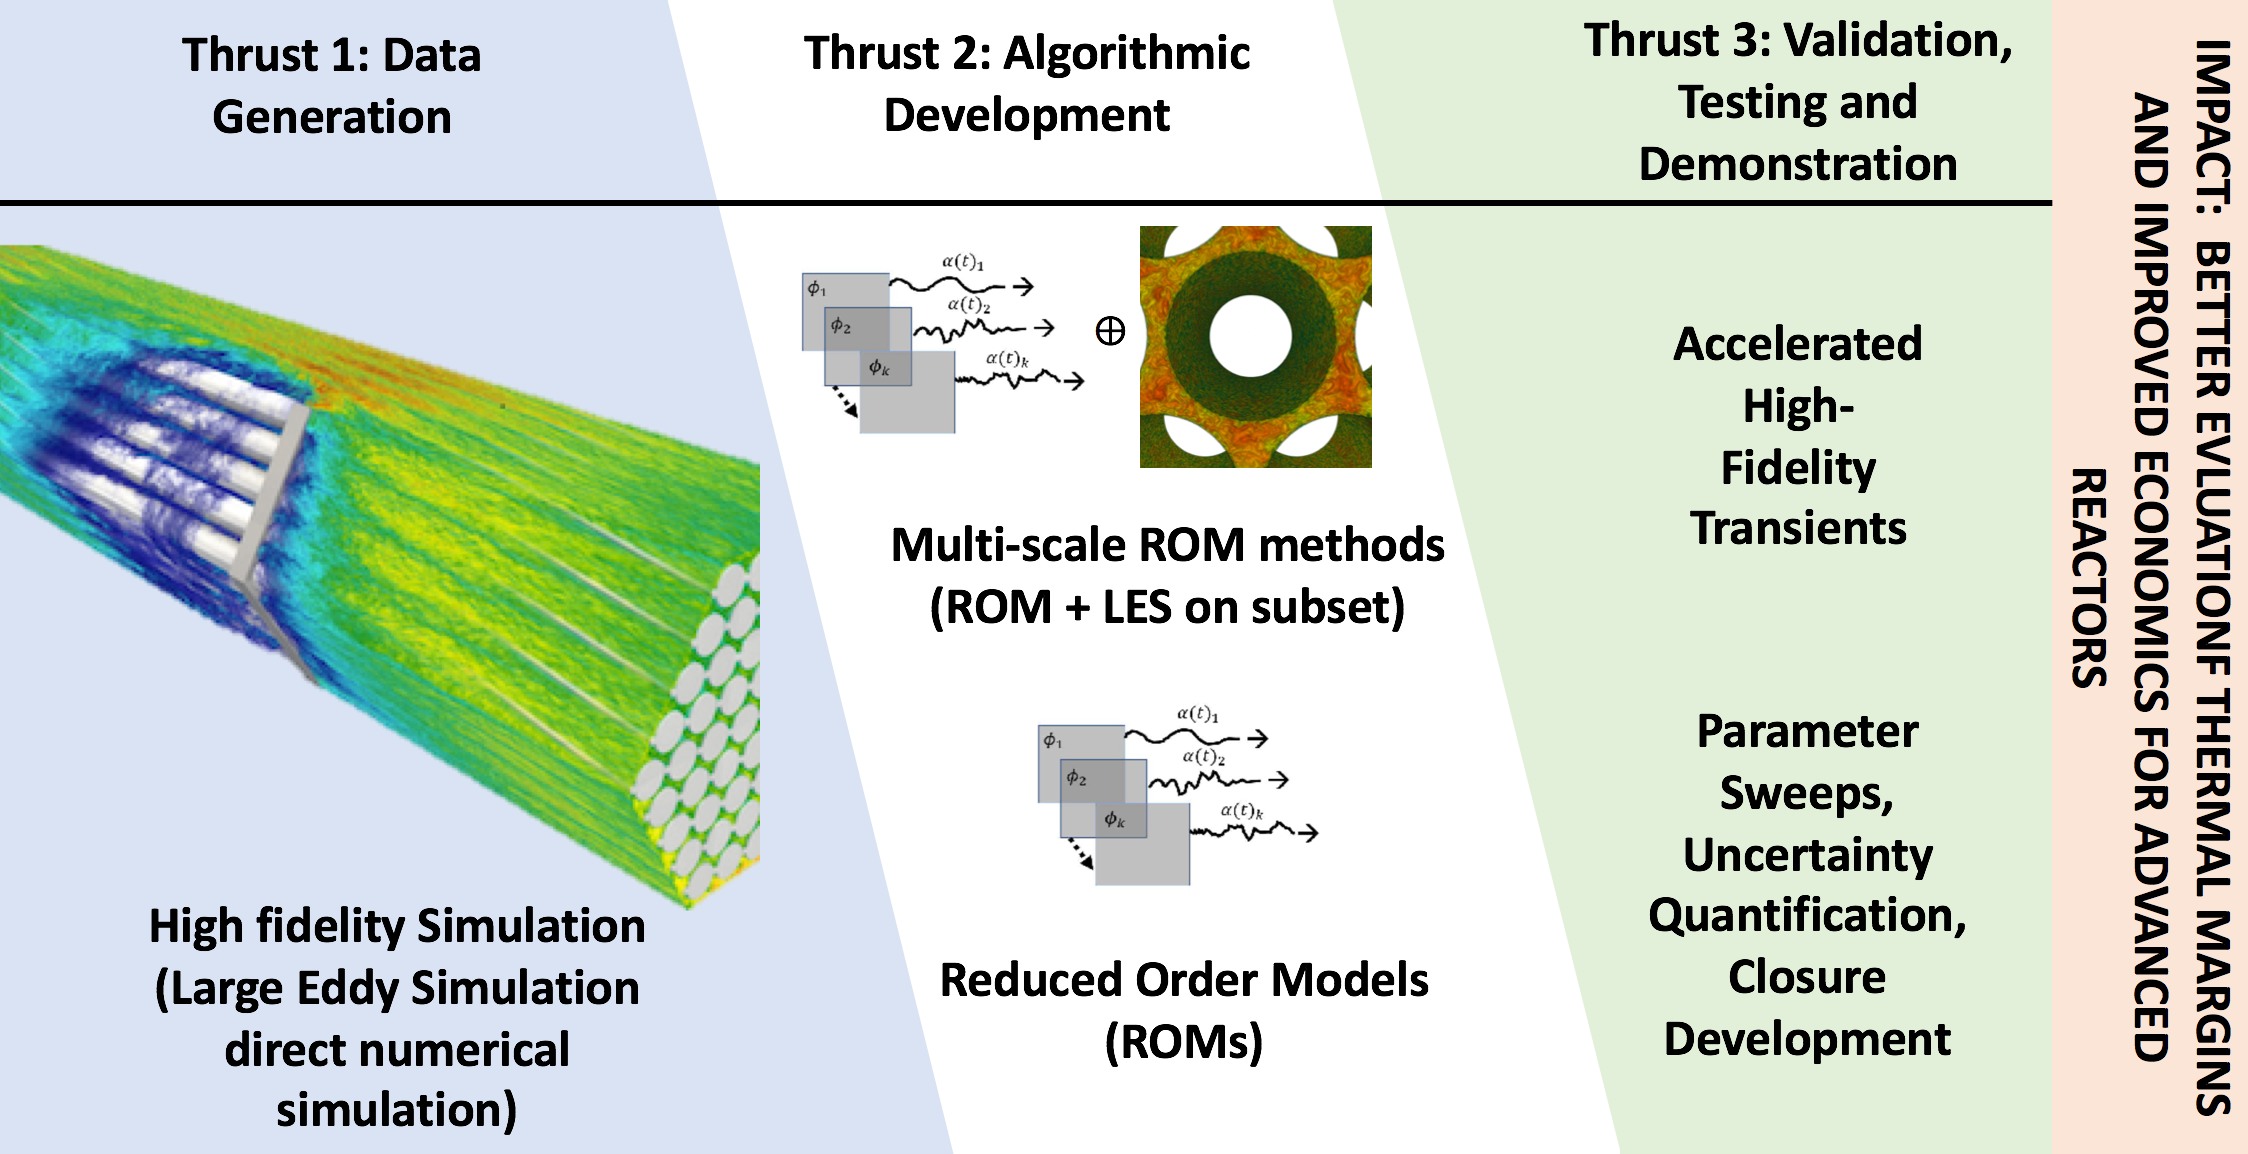
\includegraphics[height=1.78in]{figs/overview.png}}
      \put(4.20,0.00){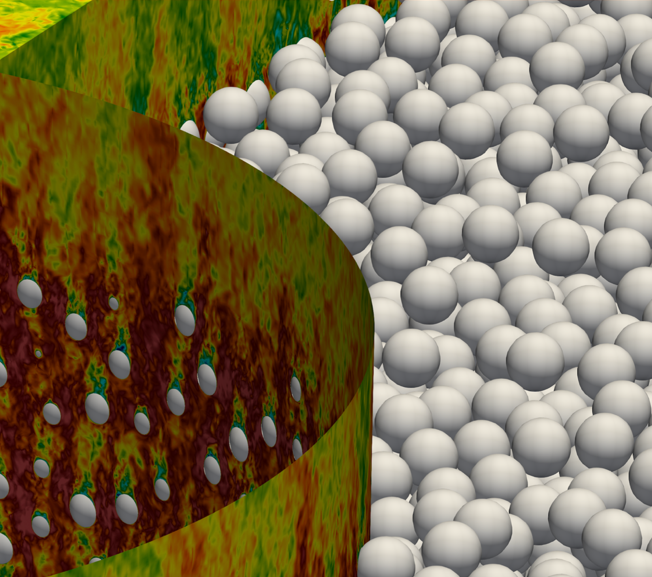
\includegraphics[height=1.78in]{figs/pbr352k_b.png}}
    \end{picture}}
    \caption{
(left) Overview of Project with three thrusts: Data Generation,
             Reduced-Order Modeling Development, and Validation/Demonstration.
(right) Current capabilities: flow-through of full pebble bed
reactor core in 6 hours on Summit. % \\[-4ex]
\label{fig:sum}}
\end{figure}

\vspace*{.0in}\noindent \underline{\textbf{Proposed Scope Description}}%  (< 1 page )
\\[-2ex]

We seek \textbf{to develop novel multi-scale algorithmic approaches for the
simulation of heat and fluid flow in advanced reactors}. The methods, which
leverage recent advances in hardware and in reduced order modeling (ROM)
approaches, will enable thermal-hydraulics (TH) simulations of vastly
accelerated speed, while maintaining accuracy comparable to high-fidelity
methods such Large Eddy Simulation (LES) and Direct Numerical Simulation (DNS).
These methods will allow designers to perform parameter sweeps to assess
uncertainty and develop closures. They will also enable, for the first time,
high fidelity simulation of long transients.

Several  advanced reactor concepts are currently being pursued in the United
States, with dozens of companies proposing unique designs. Crucial for their
deployment is the analysis of  reactor transients (e.g., a protected loss of
flow), which is an essential part of the evaluation of thermal margins and the overall
safety case.  In most cases, licensing will be pursued with established
methods, based on lumped parameter system codes (e.g., SAM \cite{hu2021}).
However, these codes require adequate closures that are typically obtained
empirically and require extensive validation. Furthermore, these methods are
characterized by high level of uncertainty when dealing with complex
three-dimensional turbulent flow, especially in the presence of large
enclosures, mixed convection, and thermal stratification. High-fidelity
simulation on the other hand remains expensive, especially for
large parameter sweeps or for the simulation of nuclear transients, and data
remains sparse.

Moreover, as the advanced reactor industry matures and moves past demonstration
projects, economics will become a larger driver. This pressure will likely push
vendors to maximize the economic potential (e.g., higher power output,
higher temperature for process heat, reduced capital cost), especially as new
materials and fuels are introduced. These goals will benefit from
improved methods to assess thermal margins that push toward high fidelity.
\textbf{This proposal seeks to develop radically novel algorithmic approaches
to the simulation of advanced reactors, with an unprecedented level of
fidelity, enabling transformative design approaches and improved economics.}
In particular we aim to: \\[-2ex]
\begin{enumerate}
%
   \item \textit{Enable the simulation of large parameter sweeps using
   ROMs developed over a subset of the parameter space.} This approach
   will allow assessment of uncertainties in system-level approaches 
   and to develop closures.
%
   \item \textit{Enable accelerated simulation of transients.}
   This approach will allow assessment of lower resolution approaches in
   conjunction with experimental data for the simulation of transients.
\\[-3ex]
\end{enumerate}
As a demonstration application we choose the simulation of Sodium Fast Reactor
(SFR) fuel assemblies under steady-state and transient conditions. \textbf{We
emphasize that the methods developed will apply to a broad range of advanced
reactor applications.} To maximize impact, we will integrate the proposed
multi-scale approaches in the Cardinal \cite{cardinal} framework thus allowing
their usage in SAM \cite{hu2021}. 

\input narrative/central

%% \vspace*{.08in}\noindent \underline{\textbf{Logical Path to Accomplishing Scope}} \\[-2ex]

\input narrative/logical

\input narrative/merit

\vspace*{.05in}\noindent \underline{\textbf{Relevance and Outcomes/Impacts}} \\[-2ex]
\input narrative/relevance

%% • Relevance and Outcomes/Impacts: This section will explain the 
%%   program relevance/priority of the effort to the objectives in the 
%%   program announcement and the expected outcomes and/or impacts.


\vspace*{.05in}\noindent \underline{\textbf{Schedule}} \\[-2ex]
\input narrative/schedule 

\vspace*{.05in}\noindent \underline{\textbf{Milestones and Deliverables}} \\[-2ex]
\input narrative/milestones 

\vspace*{.05in}\noindent \underline{\textbf{Facilities}}
% • Type/Description of facilities that will be used to execute the
%   scope (if applicable).

\input narrative/facilities

\vspace*{.05in}\noindent \underline{\textbf{Roles/Responsibilities of 
Partnering Organizations}}

\input narrative/coordination


\vspace*{.05in}\noindent \underline{\textbf{Unique Challenges}}
% Unique challenges to accomplishing the work and planned mitigations.

\textbf{THESE ARE OLD CHALLENGES}
\input narrative/uchallenge
